%% LaTeX Beamer presentation template (requires beamer package)
%% see http://bitbucket.org/rivanvx/beamer/wiki/Home
%% idea contributed by H. Turgut Uyar
%% template based on a template by Till Tantau
%% this template is still evolving - it might differ in future releases!

\documentclass{beamer}

\mode<presentation>

\usetheme{Malmoe}
\useoutertheme{infolines}
\useinnertheme{default}
\setbeamercovered{transparent}
\setbeamertemplate{footline}[frame number] % frame number in footline
\setbeamertemplate{itemize items}[circle]  % itemize circles
\renewcommand\textbullet{\ensuremath{\bullet}}  % no error for bullets
\setbeamertemplate{caption}[numbered]      % numbered captions
\beamertemplatenavigationsymbolsempty

% PACKAGES + MODIFICATIONS

\usepackage[ngerman]{babel} %language and fonts
\usepackage[utf8]{inputenc}
\usepackage{lmodern}
\usepackage{textgreek}

\usepackage{amsmath}  % math
\usepackage{amssymb}
\usepackage{mathptmx}

\usepackage{graphicx} %graphics
\usepackage{float} 
\graphicspath{{../img/}}

\usepackage{enumerate} % better way to config enumerates

\usepackage{multirow}  % multi rows in tables

\usepackage{hhline}  % for doule lines in table without interrupting vertical lines

\setbeamerfont{standard}{size=\normalsize}


% NEW COMMANDS
\newcommand{\abs}[1]{\left|#1\right|}
\newcommand{\rb}[1]{$^{#1}$\!Rb}
\newcommand{\difd}{\mathrm{d}}

% DOCUMENT SETTINGS


\title{Optisches Pumpen}
\subtitle{Fortgeschrittenen-Praktikum II}
\author{Moritz Bitterling \and Benjamin Rottler}
\institute[Universities of]{Universität Freiburg}
\date{18.05.2015}


% This is only inserted into the PDF information catalog. Can be left
% out.
\subject{Optisches Pumpen}

\AtBeginSection[]
{
\begin{frame}<beamer>[noframenumbering,plain]
\frametitle{}
\tableofcontents[currentsection,hideothersubsections]
\end{frame}
}

\begin{document}

\begin{frame}[noframenumbering,plain]
\titlepage
\end{frame}

\begin{frame}[noframenumbering,plain]
\frametitle{Inhalt}
\tableofcontents[hideallsubsections]
\end{frame}

\section{Allgemeine Grundlagen}

\subsection{Die Hyperfeinstruktur}


\begin{frame}
\frametitle{Hyperfeinstruktur-Auspaltung}
  HFS
\end{frame}


\subsection{Laser}
\begin{frame}
\frametitle{Laser}
  
\end{frame}


%\section{Laser}
\subsection{Aufbau}
\begin{frame}
\frametitle{Laser}
  
\end{frame}

\subsection{Kennlinie}

\begin{frame}
\frametitle{Kennlinie}
  
\end{frame}
%%% BEN 7.5' %%%

\section{Hyperfeinstrukturspektrum}
\subsection{Aufbau}


\begin{frame}
\frametitle{Aufbau: Bestimmung der Scanrate des Lasers}

\setbeamerfont{myfont}{size*=80}
\usebeamerfont{myfont}
\begin{figure}
    \centering
    \def\svgwidth{\textwidth}
    \input{../img/aufbauEtalon.pdf_tex}
    \caption{Aufbau zur Bestimmung der Scanrate des Lasers mit Hilfe des Etalons.}
\end{figure}



\end{frame}

\begin{frame}
\frametitle{Aufbau: Hyperfeinstrukturspektrum}

\setbeamerfont{myfont}{size*=80}
\usebeamerfont{myfont}
\begin{figure}
    \centering
    \def\svgwidth{\textwidth}
    \input{../img/aufbauHFSSpektrum.pdf_tex}
    \caption{Aufbau zur Messung des Hyperfeinstrukturspektrums.}
\end{figure}
\usebeamerfont{standard}


\begin{itemize}
  \item \textbf{Rubidiumzelle:} Füllung mit $^{85}$\!Rubidium\,+\,$^{87}$\!Rubidium (T$_\text{m}=39^\circ$C)
  und Puffergas Krypton ($p=1.5$\,mbar)
   
\end{itemize}

\end{frame}



\begin{frame}
\frametitle{Foto von Aufbau}

hier ein echtes foto

\end{frame}



\subsection{Auswertung}
\begin{frame}
\frametitle{Auswertung: Bestimmung der Scanrate des Lasers}
\begin{figure}
    \centering
    \includegraphics[width=\textwidth]{../img/down-etalon_zoom.pdf} % TODO Achsenbeschriftung
    \caption{Peaks des Etalonspektrums auf fallender Flanke.}
\end{figure}
\end{frame}

%\begin{frame}
%\frametitle{Auswertung: Bestimmung der Scanrate des Lasers}
%\begin{itemize}
%    \item<1-> Fit der Peaks mit Breit-Wigner-Verteilung und linearem Untergrund
%    \begin{equation*}
%        U_\text{ph}(t) = a_\text{ph} + b_\text{ph} \cdot t + \frac{A}{\pi} \frac{s}{s^2 + (t-x)^2}
%    \end{equation*}
%    Amplitude $A$, Zentrum $x$ und Breiteparameter $s$
%    \item<2-> Fit der Spannung für Lasermodulation mit Gerade
%\end{itemize}
%\end{frame}

\begin{frame}
\frametitle{Auswertung: Bestimmung der Scanrate des Lasers}
\begin{figure}
    \centering
    \includegraphics[width=\textwidth]{../img/down-etalon_zoom_fit.pdf}
    \caption{Fit mit Breit-Wigner-Kurven.}
\end{figure}
\end{frame}

\begin{frame}
\frametitle{Auswertung: Bestimmung der Scanrate des Lasers}
  \begin{figure}[H]
      \centering
      \includegraphics[width=\textwidth]{../img/down-etalon_zoom-etalon_calibration.pdf}
      \caption{Frequenzdifferenz der Etalonpeaks aufgetragen gegen ihre Positionen.}
  \end{figure}
\end{frame}

\begin{frame}
\frametitle{Auswertung: Bestimmung der Scanrate des Lasers}
Fit mit
\begin{equation*}
    \Delta \nu(t) = a + r \cdot t
\end{equation*}
Scanrate $r$ des Lasers
\begin{equation*}
    r = (9.47 \pm 0.08)\,\frac{\text{GHz}}{\text{ms}}
\end{equation*}
\end{frame}

\begin{frame}
\frametitle{Auswertung: Hyperfeinstruktur-Übergänge}
\begin{figure}[H]
    \centering
    \includegraphics[width=\textwidth]{../img/down-hfs.pdf}
    \caption{Hyperfeinstrukturspektrum von Rubidium.}
\end{figure}
\end{frame}

\begin{frame}
\frametitle{Auswertung: Hyperfeinstruktur-Übergänge}
\begin{figure}[H]
    \centering
    \includegraphics[width=\textwidth]{../img/down-hfs_zoom_fit.pdf}  % TODO Legend
    \caption{Hyperfeinstrukturspektrum von Rubidium mit Fit von überlagerten Gauß-Kurven.}
\end{figure}
\end{frame}

\begin{frame}
\frametitle{Auswertung: Hyperfeinstruktur-Übergänge}
\begin{equation*}
    \Delta \nu_i = r \cdot \left( \mu_i - \mu_3 \right)
\end{equation*}
\end{frame}

\begin{frame}
\frametitle{Auswertung: Hyperfeinstruktur-Übergänge}
\begin{figure}
\begin{center}
    \includegraphics[width=\textwidth]{../img/down-spectrum.pdf}
    \caption{Vergleich des auf der fallenden Flanke gemessenen Hyperfeinstrukturspektrums mit den theoretischen Werten.}
\end{center}
\end{figure}
\end{frame}

\begin{frame}
\frametitle{Auswertung: Hyperfeinstruktur-Übergänge}
\begin{itemize}[<+->]
    \item Fit mit
    \begin{equation*}
        \Delta \nu^\text{theo} = a + b \cdot \Delta \nu^\text{exp}
    \end{equation*}
    \item Ergebnis
    \begin{equation*}
        \begin{array}{ll}
            a_\text{up} = (-0.01 \pm 0.04)\,\text{GHz} & a_\text{down} = (0.05 \pm 0.04)\,\text{GHz} \\
            b_\text{up} = 0.973 \pm 0.013 & b_\text{down} = 0.970 \pm 0.013
        \end{array}
    \end{equation*}
    \item Möglicher Fehler: Etalon im Strahlengang verkippt
    \begin{itemize}[<+->]
        \item[$\Rightarrow$] Verkleinerung des freien Spektralbereichs
        \item[$\Rightarrow$] Vergrößerung der Abstände der Peaks
        \item[$\Rightarrow$] kleinere Steigung der Vergleichsgeraden
    \end{itemize}
\end{itemize}
\end{frame}

\begin{frame}
\frametitle{Auswertung: Berechnung der Intervallkonstanten $A$}
TODO Bild Termschema ohne Zeeman %TODO Termschema
\end{frame}

\begin{frame}
\frametitle{Auswertung: Berechnung der Intervallkonstanten $A$}
\begin{figure}
    \centering
    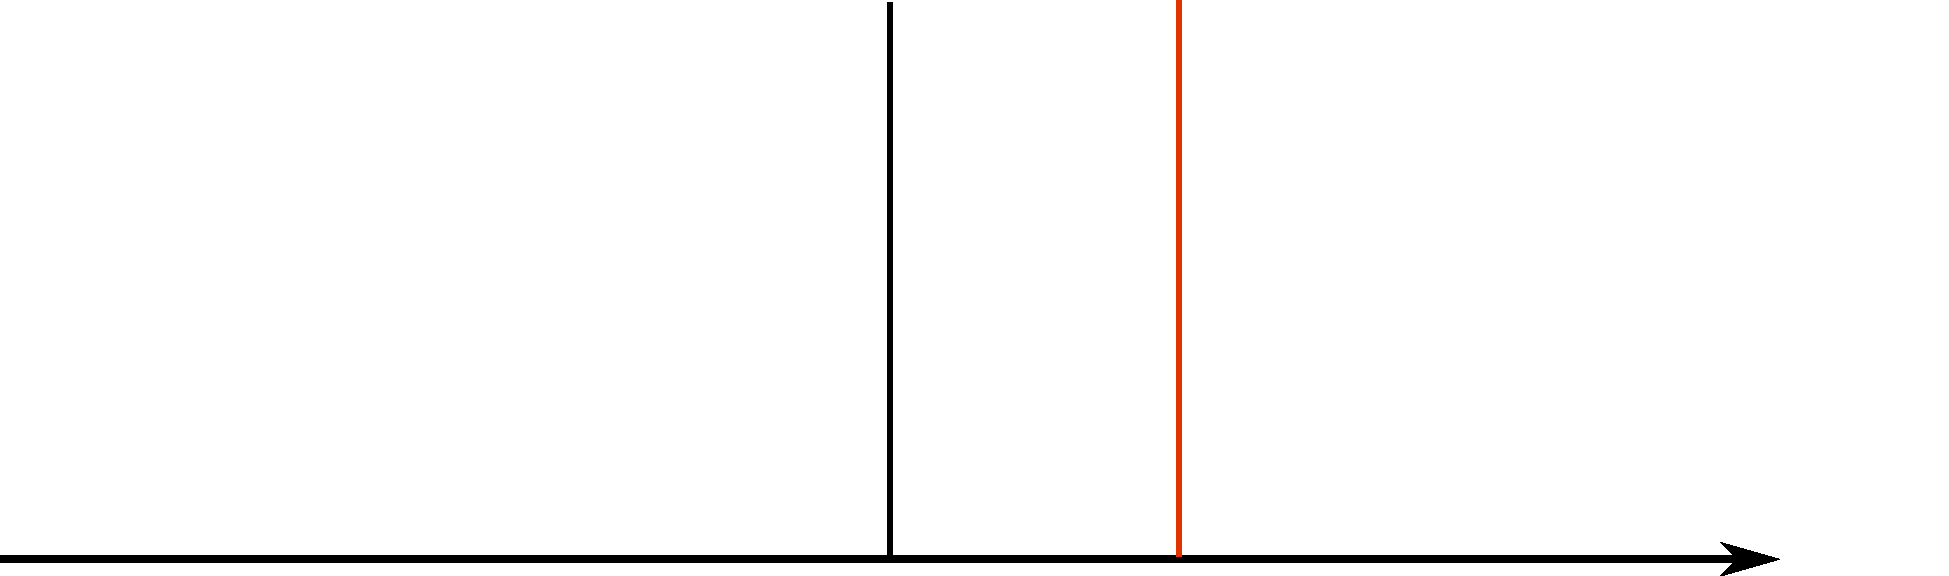
\includegraphics[width=\textwidth]{../img/HFSspect_theo.png}
    \caption{Spektrallinien der Hyperfeinstruktur des ${}^2\text{S}_{1/2}$\,-\,${}^2\text{P}_{1/2}$\,-\,Übergangs
    von \rb{85} und \rb{87}.}  % TODO Inkscape oder ref
\end{figure}
\end{frame}

\begin{frame}
\frametitle{Auswertung: Berechnung der Intervallkonstanten $A$}
\begin{equation*}
    \Delta E = \Delta \nu h = A (F + 1)
\end{equation*}
\begin{table}
\caption{Errechnete HFS-Intervallkonstanten $A$ für das ${}^2\text{S}_{1/2}$ Niveau von \rb{85} und für das ${}^2\text{S}_{1/2}$- und ${}^2\text{P}_{1/2}$ Niveau von \rb{87}.}
\begin{center}
\begin{tabular}{|c|c|c|c|}
  \hline
  Isotop / Feinstruktur & $A^\text{Lit.}$ / \textmu eV & $A^\text{exp}$ / \textmu eV & $s_{A^\text{exp}}$ / \textmu eV \\ \hline
  \rb{85}: ${}^2\text{S}_{1/2}$ & 4.185 & 4.47 & 0.14 \\ \hline
  \rb{87}: ${}^2\text{S}_{1/2}$ & 14.13 & 14.49 & 0.14 \\ \hline
  \rb{87}: ${}^2\text{P}_{1/2}$ & 1.692 & 1.61 & 0.14 \\ \hline
\end{tabular}
\end{center}
\label{tab:hfs:intervalconsts}
\end{table}
\end{frame}
%%% MORITZ 2.5' %%%

\section{Doppelresonanz}
\subsection{Grundlagen: Optisches Pumpen}


\begin{frame}
\frametitle{Optisches Pumpen}
\setbeamerfont{myfont}{size*=45}
\usebeamerfont{myfont}

  \begin{figure}
    \centering
    \def\svgwidth{0.45\textwidth}
    \input{../img/termschema.pdf_tex}
    \caption{Termschema.}
\end{figure}
\end{frame}




\begin{frame}
\frametitle{Optisches Pumpen}

\begin{figure}[H]
\begin{center}
  \includegraphics[width=\textwidth]{../img/optPumpen.png}
  \caption{ca.}
\end{center}
\end{figure}
%TODO neues Bild mit Inkscape?

\end{frame}

\subsection{Aufbau}
\begin{frame}
\frametitle{Aufbau: Doppelresonanz}

\setbeamerfont{myfont}{size*=80}
\usebeamerfont{myfont}
\begin{figure}
    \centering
    \def\svgwidth{\textwidth}
    \input{../img/aufbauDR.pdf_tex}
    \caption{Aufbau zur Messung der Doppelresonanz.}
\end{figure}
\usebeamerfont{standard}

\begin{itemize}
  \item \textbf{\textlambda/4-Plättchen:} Erzeugung von zirkular polarisiertem Licht
  \item \textbf{Spule 1:} Einstellbarer Gleichstrom
  \item \textbf{Spule 2:} Sinusförmiger Strom
  \item \textbf{Spule 4:} Kompensation von vertikalem Erdmagnetfeld
  \item \textbf{RF-Sender:} Einstrahlung von elmag. Wechselfeld in die Messzelle
\end{itemize}

\end{frame}



%%% BEN 2.5' %%%

\subsection{Auswertung}
\begin{frame}
\frametitle{Auswertung}
  
\end{frame}
%%% MORITZ 10' %%%

\section{Spinpräzession}
\subsection{Grundlagen: Spinpräzession}
\begin{frame}
\frametitle{Grundlagen}
  
\end{frame}

\subsection{Aufbau}
\begin{frame}
\frametitle{Aufbau}
  
\end{frame}

\subsection{Auswertung}
\begin{frame}
\frametitle{Auswertung}
  
\end{frame}
%%% BEN 5' %%%

\section{Dehmelt}
\subsection{Grundlagen: Dehmelt}
\begin{frame}
\frametitle{Grundlagen}
  
\end{frame}

\subsection{Aufbau}
\begin{frame}
\frametitle{Aufbau Dehmelt}

\setbeamerfont{myfont}{size*=80}
\usebeamerfont{myfont}
\begin{figure}
    \centering
    \def\svgwidth{\textwidth}
    \input{../img/aufbaudehmelt.pdf_tex}
    \caption{Aufbau..}
\end{figure}
\usebeamerfont{standard}

\begin{itemize}
  \item \textbf{ND-Filter:} Abschwächung der Laserintensität um 60\% bis 98\%
  \item \textbf{Spule 3:} Rechteckiges Wechselfeld mit 50\,Hz
  \item \textbf{Spule 4:} Kompensation von vertikalem Erdmagnetfeld
\end{itemize}

\end{frame}

\subsection{Auswertung}
\begin{frame}
\frametitle{Auswertung}
  
\end{frame}
%%% MORITZ 5' %%%

\section{Bestimmung der Relaxationszeit nach Franzen}
\subsection{Grundlagen}
\begin{frame}
\frametitle{Grundlagen: Franzen}
  
\end{frame}

\subsection{Aufbau}
\begin{frame}
\frametitle{Aufbau: Franzen}

\setbeamerfont{myfont}{size*=80}
\usebeamerfont{myfont}
\begin{figure}
    \centering
    \def\svgwidth{\textwidth}
    \input{../img/aufbaufranzen.pdf_tex}
    \caption{Aufbau..}
\end{figure}
\usebeamerfont{standard}

\begin{itemize}
  \item \textbf{Chopper:} Periodische Unterbrechung des Laserlichts
  \item \textbf{Spule 1:} Kompensation von horizontalem Erdmagnetfeld
  \item \textbf{Spule 4:} Kompensation von vertikalem Erdmagnetfeld
\end{itemize}

\end{frame}

\subsection{Auswertung}
\begin{frame}
\frametitle{Auswertung: Franzen}

\begin{figure}
    \centering
    \includegraphics[width=\textwidth]{../img/04.pdf}
    \caption{Transmission der Messzelle nach Öffnung des Strahlengangs.}  
\end{figure} 
  
\end{frame}


\begin{frame}
\frametitle{Auswertung: Franzen}

\begin{figure}
    \centering
    \includegraphics[width=\textwidth]{../img/sigmaFit.pdf}
    \caption{Abrundung der gefitteten Fermi-Funktionen.}  
\end{figure} 
  
\end{frame}


\begin{frame}
\frametitle{Auswertung: Franzen}

\begin{figure}
    \centering
    \includegraphics[width=\textwidth]{../img/BFit.pdf}
    \caption{Startwerte der gefitteten Exponentialfunktionen.}  
\end{figure} 
  
\end{frame}
%\input{template}

\end{document}
